% move all configuration stuff into includes file so we can focus on the content
\documentclass[aspectratio=169,hyperref={pdfpagelabels=false,colorlinks=true,linkcolor=white,urlcolor=blue},t]{beamer}

%%%%%%%%%%%%%%%%%%%%%%%%%%%%%%%%%%%%%%%%%%%%%%%%%%%%%%%%%%%%%%%%%%%%%%%%%%%%%%%%%%
%%%%%%%%%%%%%%%%%%%%%%%%%%%%%%%%%%%%%%%%%%%%%%%%%%%%%%%%%%%%%%%%%%%%%%%%%%%%%%%%%%
% packages
\usepackage{pict2e}
\usepackage{epic}
\usepackage{amsmath,amsfonts,amssymb}
\usepackage{units}
\usepackage{fancybox}
\usepackage[absolute,overlay]{textpos} 
\usepackage{media9} % avi2flv: "C:\Program Files\ffmpeg\bin\ffmpeg.exe" -i TuneFreqFilterbank.avi -b 600k -s 441x324 -r 15 -acodec copy TuneFreqFilterbank.flv
\usepackage{animate}
\usepackage{gensymb}
\usepackage{multirow}
\usepackage{silence}
\usepackage{tikz}
\usepackage[backend=bibtex,style=ieee]{biblatex}
\AtEveryCitekey{\iffootnote{\tiny}{}}
\addbibresource{include/references}

%%%%%%%%%%%%%%%%%%%%%%%%%%%%%%%%%%%%%%%%%%%%%%%%%%%%%%%%%%%%%%%%%%%%%%%%%%%%%%%%%%
%%%%%%%%%%%%%%%%%%%%%%%%%%%%%%%%%%%%%%%%%%%%%%%%%%%%%%%%%%%%%%%%%%%%%%%%%%%%%%%%%%
% relative paths
\graphicspath{{graph/}}


%%%%%%%%%%%%%%%%%%%%%%%%%%%%%%%%%%%%%%%%%%%%%%%%%%%%%%%%%%%%%%%%%%%%%%%%%%%%%%%%%%
%%%%%%%%%%%%%%%%%%%%%%%%%%%%%%%%%%%%%%%%%%%%%%%%%%%%%%%%%%%%%%%%%%%%%%%%%%%%%%%%%%
% units
\setlength{\unitlength}{1mm}

%%%%%%%%%%%%%%%%%%%%%%%%%%%%%%%%%%%%%%%%%%%%%%%%%%%%%%%%%%%%%%%%%%%%%%%%%%%%%%%%%%
%%%%%%%%%%%%%%%%%%%%%%%%%%%%%%%%%%%%%%%%%%%%%%%%%%%%%%%%%%%%%%%%%%%%%%%%%%%%%%%%%%
% theme & layout
\usetheme{Frankfurt}
\beamertemplatenavigationsymbolsempty
%\setbeamertemplate{frametitle}[smoothbars theme]
\setbeamertemplate{frametitle}
{
    \begin{beamercolorbox}[ht=1.8em,wd=\paperwidth]{frametitle}
        \vspace{-.1em}%
        \hspace{.2em}{\strut\insertframetitle\strut}
        
        \hspace{.2em}\small\strut\insertframesubtitle\strut
        %\hfill
        %\includegraphics[height=.8cm,keepaspectratio]{CenterMusicTechnology-solid-2lines-white-CoAtag}
        
    \end{beamercolorbox}
    \begin{textblock*}{100mm}(11.6cm,.7cm)
        \includegraphics[height=.8cm,keepaspectratio]{Logo_GTCMT_black}
    \end{textblock*}
}
\setbeamertemplate{footline}[frame number]

% set this to ensure bulletpoints without subsections
\usepackage{remreset}
\makeatletter
\@removefromreset{subsection}{section}
\makeatother
\setcounter{subsection}{1}

%---------------------------------------------------------------------------------
% appearance
\setbeamercolor{structure}{fg=gtgold}
\setbeamercovered{transparent} %invisible
\setbeamercolor{bibliography entry author}{fg=black}
\setbeamercolor*{bibliography entry title}{fg=black}
\setbeamercolor*{bibliography entry note}{fg=black}
\setbeamercolor{frametitle}{fg=black}
\setbeamercolor{title}{fg=black}

%\usepackage{pgfpages}
%\setbeameroption{show notes}
%\setbeameroption{show notes on second screen=right}
%---------------------------------------------------------------------------------
% fontsize
\let\Tiny=\tiny

%%%%%%%%%%%%%%%%%%%%%%%%%%%%%%%%%%%%%%%%%%%%%%%%%%%%%%%%%%%%%%%%%%%%%%%%%%%%%%%%%%
%%%%%%%%%%%%%%%%%%%%%%%%%%%%%%%%%%%%%%%%%%%%%%%%%%%%%%%%%%%%%%%%%%%%%%%%%%%%%%%%%%
% warnings
\pdfsuppresswarningpagegroup=1
\WarningFilter{biblatex}{Patching footnotes failed}
\WarningFilter{latexfont}{Font shape}
\WarningFilter{latexfont}{Some font shapes}
\WarningFilter{gensymb}{Not defining}


%%%%%%%%%%%%%%%%%%%%%%%%%%%%%%%%%%%%%%%%%%%%%%%%%%%%%%%%%%%%%%%%%%%%%%%%%%%%%%%%%%
%%%%%%%%%%%%%%%%%%%%%%%%%%%%%%%%%%%%%%%%%%%%%%%%%%%%%%%%%%%%%%%%%%%%%%%%%%%%%%%%%%
% theme & layout
\usetheme{Frankfurt}
\useinnertheme{rectangles}


%%%%%%%%%%%%%%%%%%%%%%%%%%%%%%%%%%%%%%%%%%%%%%%%%%%%%%%%%%%%%%%%%%%%%%%%%%%%%%%%%%
\setbeamertemplate{frametitle}[default][colsep=-4bp,rounded=false,shadow=false]
\setbeamertemplate{frametitle}
{%
    \nointerlineskip%
    %\vskip-0.5ex
    \begin{beamercolorbox}[wd=\paperwidth,ht=3.5ex,dp=0.6ex]{frametitle}
        \hspace*{1.3ex}\insertframetitle%
        
        \hspace*{1.3ex}\small\insertframesubtitle%
    \end{beamercolorbox}%
    \begin{textblock*}{100mm}(11.6cm,.57cm)
        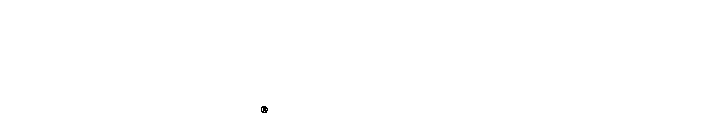
\includegraphics[height=.8cm,keepaspectratio]{graph/Logo_GTCMT_white}
    \end{textblock*}
}


%%%%%%%%%%%%%%%%%%%%%%%%%%%%%%%%%%%%%%%%%%%%%%%%%%%%%%%%%%%%%%%%%%%%%%%%%%%%%%%%%%
\setbeamertemplate{title page}[default][colsep=-4bp,rounded=false,shadow=false]
\setbeamertemplate{title page}
{
    \begin{textblock*}{100mm}(15cm,.51cm)
            \href{https://github.com/alexanderlerch/ACA-Slides/blob/2nd_edition/\jobname.pdf}{\includegraphics[height=.5cm,keepaspectratio]{graph/Logo_github}}\hspace*{2ex}
    \end{textblock*}
    \vskip-10ex
    \begin{beamercolorbox}[wd=\paperwidth,ht=.7\paperheight,dp=0.6ex]{frametitle} %35ex
        %\begin{flushright}
            %\href{http://www.gtcmt.gatech.edu}{\includegraphics[height=.8cm,keepaspectratio]{graph/Logo_GTCMT_black}}\hspace*{2ex}
        %\end{flushright}
        
        \hspace*{1.8ex}\LARGE\inserttitle%
        
        \vspace*{.5ex}
        
        \hspace*{1.3ex}\small\insertsubtitle%
        
        \vspace*{.5ex}
    \end{beamercolorbox}%
    \nointerlineskip%
    \begin{beamercolorbox}[wd=\paperwidth,ht=.4\paperheight,dp=0.6ex]{page number in head/foot}
        %\vspace*{-.5ex}
        \hspace*{1.7ex}\small\insertauthor%
        
        %\hspace*{1.7ex}\small }%
        
        \vspace*{10ex}
        
        \begin{flushright}
            \href{http://www.gtcmt.gatech.edu}{\includegraphics[height=.8cm,keepaspectratio]{graph/Logo_GTCMT_black}}\hspace*{2ex}
        \end{flushright}
    \end{beamercolorbox}%
}


%%%%%%%%%%%%%%%%%%%%%%%%%%%%%%%%%%%%%%%%%%%%%%%%%%%%%%%%%%%%%%%%%%%%%%%%%%%%%%%%%%
%\makeatother
\setbeamertemplate{footline}
{
  \leavevmode%
  \hbox{%
  \begin{beamercolorbox}[wd=.5\paperwidth,ht=2.25ex,dp=1ex,left,leftskip=1ex]{page number in head/foot}%
    \insertsubtitle
  \end{beamercolorbox}%
  \begin{beamercolorbox}[wd=.5\paperwidth,ht=2.25ex,dp=1ex,right,rightskip=1ex]{page number in head/foot}%
    \hfill
    \insertframenumber{} / \inserttotalframenumber
  \end{beamercolorbox}}%
  \vskip0pt%
}
%\makeatletter


%%%%%%%%%%%%%%%%%%%%%%%%%%%%%%%%%%%%%%%%%%%%%%%%%%%%%%%%%%%%%%%%%%%%%%%%%%%%%%%%%%
\beamertemplatenavigationsymbolsempty
\setbeamertemplate{navigation symbols}{}
\setbeamertemplate{blocks}[default]%[rounded=false,shadow=false]
\setbeamertemplate{itemize item}[square]
\setbeamertemplate{itemize subitem}[circle]
\setbeamertemplate{itemize subsubitem}[triangle]
\setbeamertemplate{enumerate item}[square]
\setbeamertemplate{enumerate subitem}[circle]
\setbeamertemplate{enumerate subsubitem}[circle]


%%%%%%%%%%%%%%%%%%%%%%%%%%%%%%%%%%%%%%%%%%%%%%%%%%%%%%%%%%%%%%%%%%%%%%%%%%%%%%%%%%
% colors
\setbeamercolor{structure}{fg=darkgray}
\setbeamercovered{transparent} %invisible
\setbeamercolor{bibliography entry author}{fg=black}
\setbeamercolor*{bibliography entry title}{fg=black}
\setbeamercolor*{bibliography entry note}{fg=black}
\setbeamercolor{frametitle}{fg=black}
\setbeamercolor{title}{fg=white}
\setbeamercolor{subtitle}{fg=white}
\setbeamercolor{frametitle}{fg=white}
\setbeamercolor{framesubtitle}{fg=white}
\setbeamercolor{mini frame}{fg=white, bg=black}
\setbeamercolor{section in head/foot}{fg=white, bg=darkgray}
\setbeamercolor{page number in head/foot}{fg=black, bg=lightblue}
\setbeamercolor{item projected}{fg=white, bg=black}

%---------------------------------------------------------------------------------
%%%%%%%%%%%%%%%%%%%%%%%%%%%%%%%%%%%%%%%%%%%%%%%%%%%%%%%%%%%%%%%%%%%%%%%%%%%%%%%%%%
%%%%%%%%%%%%%%%%%%%%%%%%%%%%%%%%%%%%%%%%%%%%%%%%%%%%%%%%%%%%%%%%%%%%%%%%%%%%%%%%%%
% title information
\title[]{Introduction to \textbf{Audio Content Analysis}}   
\author[alexander lerch]{alexander lerch} 
%\institute{~}
%\date[Alexander Lerch]{}
%\titlegraphic{\vspace{-16mm}\includegraphics[width=\textwidth,height=3cm]{title}}

%%%%%%%%%%%%%%%%%%%%%%%%%%%%%%%%%%%%%%%%%%%%%%%%%%%%%%%%%%%%%%%%%%%%%%%%%%%%%%%%%%
%%%%%%%%%%%%%%%%%%%%%%%%%%%%%%%%%%%%%%%%%%%%%%%%%%%%%%%%%%%%%%%%%%%%%%%%%%%%%%%%%%
% colors
\definecolor{gtgold}{HTML}{E0AA0F} %{rgb}{0.88,0.66,1,0.06} [234, 170, 0]/256
\definecolor{darkgray}{rgb}{.1, .1, .25}
\definecolor{lightblue}{rgb}{.1, 0.75, 1}
\definecolor{highlight}{rgb}{0, 0, 1} %_less!40

%%%%%%%%%%%%%%%%%%%%%%%%%%%%%%%%%%%%%%%%%%%%%%%%%%%%%%%%%%%%%%%%%%%%%%%%%%%%%%%%%%
%%%%%%%%%%%%%%%%%%%%%%%%%%%%%%%%%%%%%%%%%%%%%%%%%%%%%%%%%%%%%%%%%%%%%%%%%%%%%%%%%%
% relative paths
\graphicspath{{../ACA-Plots/graph/}}


%%%%%%%%%%%%%%%%%%%%%%%%%%%%%%%%%%%%%%%%%%%%%%%%%%%%%%%%%%%%%%%%%%%%%%%%%%%%%%%%%%
%%%%%%%%%%%%%%%%%%%%%%%%%%%%%%%%%%%%%%%%%%%%%%%%%%%%%%%%%%%%%%%%%%%%%%%%%%%%%%%%%%
% units
\setlength{\unitlength}{1mm}

%%%%%%%%%%%%%%%%%%%%%%%%%%%%%%%%%%%%%%%%%%%%%%%%%%%%%%%%%%%%%%%%%%%%%%%%%%%%%%%%%%
%%%%%%%%%%%%%%%%%%%%%%%%%%%%%%%%%%%%%%%%%%%%%%%%%%%%%%%%%%%%%%%%%%%%%%%%%%%%%%%%%%
% math
\DeclareMathOperator*{\argmax}{argmax}
\DeclareMathOperator*{\argmin}{argmin}
\DeclareMathOperator*{\atan}{atan}
\DeclareMathOperator*{\arcsinh}{arcsinh}
\DeclareMathOperator*{\sign}{sign}
\DeclareMathOperator*{\tcdf}{tcdf}
\DeclareMathOperator*{\si}{sinc}
\DeclareMathOperator*{\princarg}{princarg}
\DeclareMathOperator*{\arccosh}{arccosh}
\DeclareMathOperator*{\hwr}{HWR}
\DeclareMathOperator*{\flip}{flip}
\DeclareMathOperator*{\sinc}{sinc}
\DeclareMathOperator*{\floor}{floor}
\newcommand{\e}{{e}}
\newcommand{\jom}{\mathrm{j}\omega}
\newcommand{\jOm}{\mathrm{j}\Omega}
\newcommand   {\mat}[1]    		{\boldsymbol{\uppercase{#1}}}		%bold
\renewcommand {\vec}[1]    		{\boldsymbol{\lowercase{#1}}}		%bold

%%%%%%%%%%%%%%%%%%%%%%%%%%%%%%%%%%%%%%%%%%%%%%%%%%%%%%%%%%%%%%%%%%%%%%%%%%%%%%%%%%
%%%%%%%%%%%%%%%%%%%%%%%%%%%%%%%%%%%%%%%%%%%%%%%%%%%%%%%%%%%%%%%%%%%%%%%%%%%%%%%%%%
% media9
\newcommand{\includeaudio}[1]{
\href{run:audio/#1.mp3}{
\includegraphics[width=5mm, height=5mm]{graph/SpeakerIcon}}}

\newcommand{\includeanimation}[4]{{\begin{center}
                        \animategraphics[autoplay,loop,scale=.7]{#4}{animation/#1-}{#2}{#3}        
                        \end{center}
                        \addreference{matlab source: \href{https://github.com/alexanderlerch/ACA-Plots/blob/master/matlab/animate#1.m}{matlab/animate#1.m}}}
                        \inserticon{video}}
                        
%%%%%%%%%%%%%%%%%%%%%%%%%%%%%%%%%%%%%%%%%%%%%%%%%%%%%%%%%%%%%%%%%%%%%%%%%%%%%%%%%%
%%%%%%%%%%%%%%%%%%%%%%%%%%%%%%%%%%%%%%%%%%%%%%%%%%%%%%%%%%%%%%%%%%%%%%%%%%%%%%%%%%
% other commands
\newcommand{\question}[1]{%\vspace{-4mm}
                          \setbeamercovered{invisible}
                          \begin{columns}[T]
                            \column{.9\textwidth}
                                \textbf{#1}
                            \column{.1\textwidth}
                                \vspace{-8mm}
                                \begin{flushright}
                                     
\includegraphics[width=.9\columnwidth]{graph/question_mark}
                                \end{flushright}
                                \vspace{6mm}
                          \end{columns}\pause\vspace{-12mm}}

\newcommand{\toremember}[1]{
                        \inserticon{lightbulb}
                        }

\newcommand{\matlabexercise}[1]{%\vspace{-4mm}
                          \setbeamercovered{invisible}
                          \begin{columns}[T]
                            \column{.8\textwidth}
                                \textbf{matlab exercise}: #1
                            \column{.2\textwidth}
                                \begin{flushright}
                                     \includegraphics[scale=.5]{graph/logo_matlab}
                                \end{flushright}
                                %\vspace{6mm}
                          \end{columns}}

\newcommand{\addreference}[1]{  
                  
                    \begin{textblock*}{\baselineskip }(.98\paperwidth,.5\textheight) %(1.15\textwidth,.4\textheight)
                         \begin{minipage}[b][.5\paperheight][b]{1cm}%
                            \vfill%
                             \rotatebox{90}{\tiny {#1}}
                        \end{minipage}
                   \end{textblock*}
                    }
                    
\newcommand{\figwithmatlab}[1]{
                    \begin{figure}
                        \centering
                        \includegraphics[scale=.7]{#1}
                        %\label{fig:#1}
                    \end{figure}
                    
                    \addreference{matlab source: \href{https://github.com/alexanderlerch/ACA-Plots/blob/main/matlab/plot#1.m}{plot#1.m}}}
\newcommand{\figwithref}[2]{
                    \begin{figure}
                        \centering
                        \includegraphics[scale=.7]{#1}
                        \label{fig:#1}
                    \end{figure}
                    
                    \addreference{#2}}  
                                    
\newcommand{\inserticon}[1]{
                    \begin{textblock*}{100mm}(14.5cm,7.5cm)
                        \includegraphics[height=.8cm,keepaspectratio]{graph/#1}
                    \end{textblock*}}            

%%%%%%%%%%%%%%%%%%%%%%%%%%%%%%%%%%%%%%%%%%%%%%%%%%%%%%%%%%%%%%%%%%%%%%%%%%%%%%%%%%
%%%%%%%%%%%%%%%%%%%%%%%%%%%%%%%%%%%%%%%%%%%%%%%%%%%%%%%%%%%%%%%%%%%%%%%%%%%%%%%%%%
% counters
\newcounter{i}
\newcounter{j}
\newcounter{iXOffset}
\newcounter{iYOffset}
\newcounter{iXBlockSize}
\newcounter{iYBlockSize}
\newcounter{iYBlockSizeDiv2}
\newcounter{iXBlockSizeDiv2}
\newcounter{iDistance}




\subtitle{Module 10.1: Alignment~---~Dynamic Time Warping}

%%%%%%%%%%%%%%%%%%%%%%%%%%%%%%%%%%%%%%%%%%%%%%%%%%%%%%%%%%%%%%%%%%%%%%%%%%%%
\begin{document}
    % generate title page
	{
\setbeamertemplate{headline}{} 
\setbeamertemplate{footline}{} 
\begin{frame}
    \titlepage
    %\vspace{-5mm}
\end{frame}
}
\addtocounter{framenumber}{-1}


    \section[overview]{lecture overview}
        \begin{frame}{introduction}{overview}
            \begin{block}{corresponding textbook section}
                    %\href{http://ieeexplore.ieee.org/xpl/articleDetails.jsp?arnumber=6331124}{Chapter 7: Alignment} (pp.~139--146)
                    Section~10.1
            \end{block}

            \begin{itemize}
                \item   \textbf{lecture content}
                    \begin{itemize}
                        \item   Dynamic Time Warping (DTW):
                        \item[] synchronization of two sequences with similar content
                    \end{itemize}
                \bigskip
                \item<2->   \textbf{learning objectives}
                    \begin{itemize}
                        \item   explain the standard DTW algorithm
                        \item   discuss disadvantages of and modifications to the standard DTW algorithm
                        \item   implement DTW
                    \end{itemize}
            \end{itemize}
            \inserticon{directions}
        \end{frame}

    \section[intro]{introduction}
        \begin{frame}{dynamic time warping}{problem statement}
            \begin{columns}[T]
            \column{.5\linewidth}
            \begin{itemize}
                \item   \textbf{synchronize two sequences}
                    \begin{itemize}
                        \item	\textit{similar} musical content
                        \item	\textit{different} tempo and timing
                            \begin{footnotesize}
                            \[A(n_\mathrm{A})\quad n_\mathrm{A} \in [0;\mathcal{N}_\mathrm{A}-1]\]
                            \[B(n_\mathrm{B})\quad n_\mathrm{B} \in [0;\mathcal{N}_\mathrm{B}-1]\]
                            %\begin{itemize}
                                %\item[]	$$
                                %\item[]	$$
                            %\end{itemize}
                            \end{footnotesize}
                        \bigskip
                        \item[$\Rightarrow$] find alignment path 
                            \begin{itemize}
                                \item   minimizing pairwise distance between sequences
                                \item   covering whole sequence
                                \item   moving only forward in time
                            \end{itemize}
                    \end{itemize}
                \end{itemize}
            \column{.5\linewidth}
                \figwithmatlab{SequenceAlignment}
                %\begin{figure}
                    %\includegraphics[width=\columnwidth]{SequenceAlignment}
                %\end{figure}
            \end{columns}
            %\addreference{matlab source: \href{https://github.com/alexanderlerch/ACA-Slides/blob/master/matlab/displaySequenceAlignment.m}{matlab/displaySequenceAlignment.m}}
        \end{frame}
    \section[DTW]{dynamic time warping}
        \begin{frame}{dynamic time warping}{overview}
            \begin{itemize}
                \item   dynamic programming technique
                \smallskip
                \item   time is warped non-linearly to match sequences
                \smallskip
                \item   finds optimal match between two sequences given a cost function
                \smallskip
                \item   the overall cost indicates the overall distance between the sequences
            \end{itemize}
        \end{frame}
        \begin{frame}{dynamic time warping}{processing steps}
            \vspace{-3mm}
            \begin{columns}[T]
            \column{.4\linewidth}
                \begin{enumerate}
                    \item   extract suitable \textbf{features}\\ $\Rightarrow$ two series of feature vectors
                    \smallskip
                    \item<1->	compute \textbf{distance matrix}\\ $\mat{D}_{\mathrm{AB}}(n_\mathrm{A},n_\mathrm{B})$
                    \smallskip
                    \item<1->	compute \textbf{alignment path}\\ $\vec{P}(n_\mathrm{P})$ with $n_\mathrm{P} \in
                [0;\mathcal{N}_{\mathrm{P}}-1]$
                        \begin{itemize}
                            \item[$\Rightarrow$]	minimal \textit{overall} distance
                        \end{itemize}
                    \smallskip
                    \item<1->   (align sequences using dynamic time stretching)
                \end{enumerate}
            \column{.6\linewidth}
                \vspace{-7mm}
                \figwithmatlab{DtwPath}
                %\begin{figure}
                    %\includegraphics[width=\columnwidth]{SimMatrix}
                %\end{figure}
            \end{columns}
            %\addreference{matlab source: \href{https://github.com/alexanderlerch/ACA-Slides/blob/master/matlab/displaySimMatrix.m}{matlab/displaySimMatrix.m}}
        \end{frame}
    \section[distance]{distance matrix}
        \begin{frame}{dynamic time warping}{distance matrix computation}
            %given 2 sequences of vectors, compute the distance between all pairs of observations
           \vspace{-3mm}
            \begin{columns}[T]
            \column{.4\linewidth}
                \begin{itemize}
                    \item   given 2 sequences of vectors, compute the distance between all pairs of observations
                    \smallskip
                    \item<1->	compute distance matrix\\ $\mat{D}_{\mathrm{AB}}(n_\mathrm{A},n_\mathrm{B})$
                    \smallskip
                        \begin{itemize}
                            \item   example  $\mat{D}_{\mathrm{AB}}(1,n_\mathrm{B})$ is the distance of the first vector in Seq.\ A to all vectors in Seq.\ B
                        \end{itemize}
                \end{itemize}
            \column{.6\linewidth}
                \vspace{-7mm}
                \figwithmatlab{DtwPath}
            \end{columns}
            %\addreference{matlab source: \href{https://github.com/alexanderlerch/ACA-Slides/blob/master/matlab/displaySimMatrix.m}{matlab/displaySimMatrix.m}}
        \end{frame}
    \section[path]{path}
        \begin{frame}{dynamic time warping}{path properties 1/2}
            \begin{itemize}
                    \item	\textbf{boundaries}: covers both $A,B$ from beginning to end
                            \begin{eqnarray*}
                                \vec{P}(0) 		&=& [0, 0] \\
                                \vec{P}(\mathcal{N}_{\mathrm{P}}-1) 	&=& [\mathcal{N}_\mathrm{A}-1, \mathcal{N}_\mathrm{B}-1] 
                            \end{eqnarray*}
                    
                    \item<2->	\textbf{causality}: only forward movement
                            \begin{eqnarray*}
                                n_\mathrm{A}\big|_{\vec{P}(n_\mathrm{P})} \leq n_\mathrm{A}\big|_{\vec{P}(n_\mathrm{P}+1)} \\ 
                                n_\mathrm{B}\big|_{\vec{P}(n_\mathrm{P})} \leq n_\mathrm{B}\big|_{\vec{P}(n_\mathrm{P}+1)} 
                            \end{eqnarray*}
                    
                    \item<3->	\textbf{continuity}: no jumps
                            \begin{eqnarray*}
                                n_\mathrm{A}\big|_{\vec{P}(n_\mathrm{P}+1)} \leq (n_\mathrm{A}+1)\big|_{\vec{P}(n_\mathrm{P})} \\ 
                                n_\mathrm{B}\big|_{\vec{P}(n_\mathrm{P}+1)} \leq (n_\mathrm{B}+1)\big|_{\vec{P}(n_\mathrm{P})} 
                            \end{eqnarray*}
            \end{itemize}
        \end{frame}
        \begin{frame}{alignment}{path properties 2/2}
                \begin{figure}
                    \input{pict/alignment_warppath}
                \end{figure}

                \question{what is the minimum/maximum path length}
                    \begin{equation*}
                        \mathcal{N}_\mathrm{P, min} = \max(\mathcal{N}_\mathrm{A}, \mathcal{N}_\mathrm{B})
                    \end{equation*}
                    \begin{equation*}
                        \mathcal{N}_\mathrm{P, max} = \mathcal{N}_\mathrm{A} + \mathcal{N}_\mathrm{B} - 2
                    \end{equation*}
        \end{frame}
        
    \section[cost]{cost matrix}
        \begin{frame}{alignment}{DTW: overall cost}
            \begin{itemize}
                \item	every path has an \textit{overall cost}
                    \begin{equation*}
                        \mathfrak{C}_{\mathrm{AB}}(j) = \sum\limits_{n_\mathrm{P}= 0}^{\mathcal{N}_{\mathrm{P}}-1}{\mat{D}\big(\vec{P}_j(n_\mathrm{P})\big)} 
                    \end{equation*}
                \item<2->	\textit{optimal} path minimizes the overall cost
                    \begin{eqnarray*}
                        \mathfrak{C}_{\mathrm{AB},min} &=& \min\limits_{\forall j}\big(\mathfrak{C}_{\mathrm{AB}}(j)\big) \\
                        j_\mathrm{opt} 				&=& \argmin\limits_{\forall j}\big(\mathfrak{C}_{\mathrm{AB}}(j)\big) 
                    \end{eqnarray*}
                \item[$\Rightarrow$]<2-> stay in the 'valleys' of distance matrix
            \end{itemize}
            \question{how to determine the optimal path}
        \end{frame}
        \begin{frame}{alignment}{DTW: accumulated cost 1/2}
            accumulated cost: \textit{cost matrix}
                \begin{equation*}\label{eq:acccost}
                            \mat{C}_{\mathrm{AB}}(n_\mathrm{A},n_\mathrm{B}) = \mat{D}_{\mathrm{AB}}(n_\mathrm{A},n_\mathrm{B}) + \min\left\{
                                                    \begin{array}{llr} 
                                                        \mat{C}_{\mathrm{AB}}(n_\mathrm{A}-1, n_\mathrm{B}-1)\\
                                                        \mat{C}_{\mathrm{AB}}(n_\mathrm{A}-1, n_\mathrm{B}) \\
                                                        \mat{C}_{\mathrm{AB}}(n_\mathrm{A},	n_\mathrm{B}-1)
                                                    \end{array} 
                                                    \right. 
                \end{equation*}
                \begin{itemize}
                    \item	initialization
                        \begin{equation*}
                            \mat{C}_{\mathrm{AB}}(0,0) 	= \mat{D}_{\mathrm{AB}}(0,0) 
                        \end{equation*}
                \end{itemize}
                \begin{figure}
                    \input{pict/alignment_warppath}
                \end{figure}
        \end{frame}
        \begin{frame}{alignment}{DTW: accumulated cost 2/2}
            \vspace{-5mm}
            \figwithmatlab{DtwCost}
        \end{frame}
        \begin{frame}{alignment}{DTW: algorithm description 1/2}
                \begin{itemize}
                    \item	\textbf{initialization}:
                        \begin{footnotesize}
                            \begin{equation*}
                                \mat{C}_{\mathrm{AB}}(0,0) = \mat{D}_{\mathrm{AB}}(0,0) ,
                                \mat{C}_{\mathrm{AB}}(n_\mathrm{A},-1) = \infty ,
                                \mat{C}_{\mathrm{AB}}(-1,n_\mathrm{B}) = \infty \nonumber
                            \end{equation*}
                        \end{footnotesize}
                    \item<2->	\textbf{recursion}:
                        \begin{footnotesize}
                            \begin{eqnarray*}
                                \mat{C}_{\mathrm{AB}}(n_\mathrm{A},n_\mathrm{B}) &=& \mat{D}_{\mathrm{AB}}(n_\mathrm{A},n_\mathrm{B}) + \min\left\{
                                                            \begin{array}{l} 
                                                                \mat{C}_{\mathrm{AB}}(n_\mathrm{A}-1, n_\mathrm{B}-1)\\
                                                                \mat{C}_{\mathrm{AB}}(n_\mathrm{A}-1, n_\mathrm{B}) \\
                                                                \mat{C}_{\mathrm{AB}}(n_\mathrm{A},	n_\mathrm{B}-1)
                                                            \end{array} 
                                                            \right. \\
                                j &=& \argmin\left\{
                                                            \begin{array}{l} 
                                                                \mat{C}_{\mathrm{AB}}(n_\mathrm{A}-1, n_\mathrm{B}-1)\\
                                                                \mat{C}_{\mathrm{AB}}(n_\mathrm{A}-1, n_\mathrm{B}) \\
                                                                \mat{C}_{\mathrm{AB}}(n_\mathrm{A},	n_\mathrm{B}-1)
                                                            \end{array} 
                                                            \right. \\
                                \Delta\vec{P}(n_\mathrm{A},n_\mathrm{B}) &=& \left\{ 
                                                            \begin{array}{ll} 
                                                              [-1, -1] &\mbox{if }	j = 0 \\{} 
                                                              [-1, 0] &\mbox{if }	j = 1 \\{}
                                                              [0, -1] &\mbox{if }	j = 2  
                                                            \end{array} 
                                                            \right.
                            \end{eqnarray*}
                        \end{footnotesize}
                \end{itemize}
        \end{frame}
        \begin{frame}{alignment}{DTW: algorithm description 2/2}
                \begin{itemize}
                    \item	\textbf{termination}:
                        \begin{footnotesize}
                            \begin{equation*}
                                n_\mathrm{A}= \mathcal{N}_\mathrm{A}-1 \wedge n_\mathrm{B} = \mathcal{N}_\mathrm{B}-1 
                            \end{equation*}
                        \end{footnotesize}
                    \bigskip
                    \item<2->	\textbf{path backtracking}:
                        \begin{footnotesize}
                            \begin{equation*}
                                \vec{P}(n_\mathrm{P}) = \vec{P}(n_\mathrm{P}+1) + \Delta\vec{P}\big(\vec{P}(n_\mathrm{P}+1)\big), \;n_\mathrm{P} = \mathcal{N}_{\mathrm{P}}-2, \mathcal{N}_{\mathrm{P}}-3,\ldots, 0 \nonumber
                            \end{equation*}
                        \end{footnotesize}
                \end{itemize}
        \end{frame}
    \section{example}
        \begin{frame}{dynamic time warping}{DTW: example}
            \begin{textblock*}{100mm}(1cm,2.5cm)
                \includegraphics[scale=.25]{SequenceAlignment}
            \end{textblock*}
            \vspace{-5mm}
            \figwithmatlab{DtwPath}
        \end{frame}
        \begin{frame}{dynamic time warping}{example}
            \begin{eqnarray*}
                A &=& [1,\ 2,\ 3,\ 0] ,\nonumber\\
                B &=& [1,\ 0,\ 2,\ 3,\ 1] ,\nonumber
            \end{eqnarray*}
            \question{compute distance matrix, cost matrix, and DTW path}
                    \begin{equation*}
                        \only<2-3>{
                        \mat{D}_{\mathrm{AB}} =   \left[ 
                                        \begin{array}{cccc}
                                        0					&	\color{black}{1}	&	\color{black}{2}	&	\color{black}{1}\\
                                        1					&	\color{black}{2}	&	\color{black}{3}	&	\color{black}{0}\\
                                        \color{black}{1}	&	0 					&	\color{black}{1}	&	\color{black}{2}\\
                                        \color{black}{2}	&	\color{black}{1}	&	0							&	\color{black}{3}\\
                                        \color{black}{0}	&	\color{black}{1}	&	\color{black}{2}	&	1\\
                                    \end{array}  
                                \right]
                                \quad\quad
                        \visible<3>{
                        \mat{C}_{\mathrm{AB}} =   \left[ 
                                        \begin{array}{cccc}
                                        0					&	\leftarrow\color{black}{1}	&	\leftarrow\color{black}{3}	&	\leftarrow\color{black}{4}\\
                                        \uparrow 1					&	\nwarrow\color{black}{2}	&	\nwarrow\color{black}{4}	&	\nwarrow\color{black}{3}\\
                                        \uparrow\color{black}{2}	&	\nwarrow 1 					&	\leftarrow\color{black}{2}	&	\leftarrow\color{black}{4}\\
                                        \uparrow\color{black}{4}	&	\uparrow\color{black}{2}	&	\nwarrow 1							&	\leftarrow\color{black}{4}\\
                                        \uparrow\color{black}{4}	&	\uparrow\color{black}{3}	&	\uparrow\color{black}{3}	&	\nwarrow 2\\
                                    \end{array}  
                                \right]  
                                }
                                }
                        \only<4>{
                    \mat{D}_{\mathrm{AB}} =   \left[ 
                                    \begin{array}{cccc}
                                    \color{highlight}{0}			&	\textcolor[gray]{0.6}{1}	&	\textcolor[gray]{0.6}{2}	&	\textcolor[gray]{0.6}{1}\\
                                    \color{highlight}{1}			&	\textcolor[gray]{0.6}{2}	&	\textcolor[gray]{0.6}{3}	&	\textcolor[gray]{0.6}{0}\\
                                    \textcolor[gray]{0.6}{1}	&	\color{highlight}{0} 			&	\textcolor[gray]{0.6}{1}	&	\textcolor[gray]{0.6}{2}\\
                                    \textcolor[gray]{0.6}{2}	&	\textcolor[gray]{0.6}{1}	&	\color{highlight}{0}			&	\textcolor[gray]{0.6}{3}\\
                                    \textcolor[gray]{0.6}{0}	&	\textcolor[gray]{0.6}{1}	&	\textcolor[gray]{0.6}{2}	&	\color{highlight}{1}\\
                                \end{array}  
                            \right]  
                                \quad\quad
                        \mat{C}_{\mathrm{AB}} =   \left[ 
                                        \begin{array}{cccc}
                                        \color{highlight}{0}       	&	\leftarrow\textcolor[gray]{0.6}{1}	&	\leftarrow\color[gray]{0.6}{3}	&	\leftarrow\color[gray]{0.6}{4}\\
                                        \color{highlight}{\uparrow 1}	&	\nwarrow\color[gray]{0.6}{2}	&	\nwarrow\color[gray]{0.6}{4}	&	\nwarrow\color[gray]{0.6}{3}\\
                                        \uparrow\color[gray]{0.6}{2}	&	\color{highlight}{\nwarrow 1}  &	\leftarrow\color[gray]{0.6}{2}	&	\leftarrow\color[gray]{0.6}{4}\\
                                        \uparrow\color[gray]{0.6}{4}	&	\uparrow\color[gray]{0.6}{2}	&	\color{highlight}{\nwarrow 1}  &	\leftarrow\color[gray]{0.6}{4}\\
                                        \uparrow\color[gray]{0.6}{4}	&	\uparrow\color[gray]{0.6}{3}	&	\uparrow\color[gray]{0.6}{3}	&	\color{highlight}{\nwarrow 2}\\
                                    \end{array}  
                                \right]  
                                }
                    \end{equation*}
        \end{frame}
        %\begin{frame}{alignment}{DTW: matlab implementation}
            %\matlabexercise{implement a DTW function in Matlab}
            %
            %\begin{enumerate}
                %\item   create a function with the interface\\ \texttt{function [p, C] = SimpleDtw(D)}
                    %\begin{itemize}
                        %\item   $p$: path through matrix ($\mathcal{N}_P\times 2$)
                        %\item   $C$: cost matrix (same dimension as $D$)
                        %\item   $D$: distance matrix ($\mathcal{N}_B\times \mathcal{N}_A$)
                    %\end{itemize}
                %\item   your function should contain 3 major code blocks
                    %\begin{itemize}
                        %\item   initialization
                        %\item   cost matrix computation
                        %\item   back-tracking for extracting the path indices
                    %\end{itemize}
                %\item   what would be a proper test case to validate your implementation
            %\end{enumerate}
        %\end{frame}
    \section[variants]{DTW variants}
        \begin{frame}{dynamic time warping}{variants}
            \begin{itemize}
                \item	transition weights: favor specific path directions
                    \begin{footnotesize}
                        \begin{equation*}
                            \mat{C}_{\mathrm{AB}}(n_\mathrm{A},n_\mathrm{B}) = \min\left\{
                                                    \begin{array}{lll} 
                                                    \mat{C}_{\mathrm{AB}}(n_\mathrm{A}-1,n_\mathrm{B}-1)	&+& \lambda_\mathrm{d}\cdot\mat{D}_{\mathrm{AB}}(n_\mathrm{A},n_\mathrm{B})\\
                                                    \mat{C}_{\mathrm{AB}}(n_\mathrm{A}-1,n_\mathrm{B}) 	&+& \lambda_\mathrm{v}\cdot\mat{D}_{\mathrm{AB}}(n_\mathrm{A},n_\mathrm{B})\\
                                                    \mat{C}_{\mathrm{AB}}(n_\mathrm{A},n_\mathrm{B}-1) 	&+& \lambda_\mathrm{h}\cdot\mat{D}_{\mathrm{AB}}(n_\mathrm{A},n_\mathrm{B})
                                                    \end{array} 
                                                    \right.\nonumber
                        \end{equation*}
                    \end{footnotesize}
                \item<2->	step types
                \begin{figure}
                    \input{pict/alignment_warppathoptions}
                \end{figure}
                
            \end{itemize}
        \end{frame}
        \begin{frame}{dynamic time warping}{optimization}
            \vspace{-3mm}
            \begin{itemize}
                \item \textbf{challenge}:  distance matrix dimensions  $\mathcal{N}_\mathrm{A}\cdot \mathcal{N}_\mathrm{B}$
                \smallskip
                \item[$\Rightarrow$] DTW \textit{inefficient} for long sequences 
                    \begin{itemize}
                        \item	high memory requirements
                        \item	large number of operations
                    \end{itemize}
            \end{itemize}
            \vspace{-2mm}
            \begin{columns}
            \column{.4\linewidth}
                 
                    \begin{enumerate}
                        \item<2->[] \textbf{optimizations}: 
                        \item<2->	maximum time and tempo deviation
                        \item<3->	sliding window 
                        \item<4->	multi-scale DTW (several downsampled iterations)
                    \end{enumerate}
            \column{.6\linewidth}
                \only<2>{
                    \figwithmatlab{DtwConstraints}
                }
                \only<3>{
                    \vspace{-4mm}
                    \begin{figure}
                        \centerline{\includegraphics[scale=.3]{graph/dtw_match}}
                    \end{figure}
                }
                \only<4>{
                    \vspace{-4mm}
                    \begin{figure}
                        \centerline{\includegraphics[scale=.4]{graph/multiscaledtw}}
                    \end{figure}
                }
            \end{columns}
            \vspace{-2mm}
            \only<3>{\footfullcite{dixon_match:_2005}}
            \only<4>{\footfullcite{muller_efficient_2006}}
        \end{frame}

    
    \section{summary}
        \begin{frame}{dynamic time warping}{DTW vs.\ Viterbi}
            \question{similarities and differences of DTW and the Viterbi algorithm}
              
                \bigskip
                \begin{itemize}
                    \item   \textbf{commonalities}
                        \begin{itemize}
                            \item   find path through matrix 
                            \item   maximizes overall probability/minimizes overall cost
                            \item   based on dynamic programming principles
                        \end{itemize}
                    \smallskip
                    \item   \textbf{differences}
                        \begin{itemize}
                            \item   DTW has more constraints: start/end in corner, move only to neighbor
                            \item   DTW is not usually parametrized by training data (transition probs, construction of distance/emission prob matrix)
                            \item   Viterbi path length is predefined, DTW path length is not
                        \end{itemize}
                \end{itemize}
        \end{frame}
        \begin{frame}{summary}{lecture content}
            \begin{itemize}
                \item   \textbf{dynamic time warping}
                    \begin{itemize}
                        \item   find globally optimal alignment path between two sequences
                    \end{itemize}
                \bigskip
                \item   \textbf{processing steps}
                    \begin{enumerate}
                        \item   compute distance matrix
                        \item   compute cost matrix
                        \item   back-track path
                    \end{enumerate}
            \end{itemize}
            \inserticon{summary}
        \end{frame}
\end{document}
